%! TEX program = xelatex
\documentclass[10pt]{beamer}


\usetheme[progressbar=frametitle]{metropolis}
\setsansfont[BoldFont={Fira Sans}]{Fira Sans Light}
\setmonofont{Fira Mono}
\usepackage{appendixnumberbeamer}

\usepackage{booktabs}
\usepackage[scale=2]{ccicons}

\title{Tecniche di animazione 3D nella realizzazione di un cortometraggio}
\subtitle{Elaborato in Computer Grafica}						% L'obiettivo della mia tesi è quello di realizzare un cortometraggio animato in 3D con l'utilizzo della computer grafica.
% \date{\today}                                     % Ho scelto questo ambito perché è in linea col Master, che ho iniziato in Svezia, sulla visualizzazione e la grafica interattiva.
\date{10 Dicembre 2019}
\author{Leonardo Marini}
\institute{ALMA MATER STUDIORUM - UNIVERSITÀ DI BOLOGNA}
%\titlegraphic{\hfill
\includegraphics[height=1.5cm]{logo.pdf}}

\begin{document}

\maketitle

\begin{frame}{Indice}																		% Il progetto ha incluso una fase di analisi per capire quali fossero i requisiti.
  \setbeamertemplate{section in toc}[sections numbered] % Ad una di progettazione in cui sono si sono decise le diverse tecniche da usare poi nella produzione.
  \tableofcontents%[hideallsubsections]									% Le tecniche sono state quindi analizzate e studiate da un punto di vista principalmente matematico.
\end{frame}

\section[Intro]{Introduzione}

\begin{frame}{Analisi} 
      \begin{itemize}[<+- | alert@+>]								% Tra i requisiti abbiamo che il
        \item Cortometraggio animato in 3D 					% cortometraggio dev'essere realizzato in 3D con l'uso della computer grafica.
        \item Uso di diverse tecniche di animazione % Devono essere usate diverse tecniche di animazione 3D.
        \item Breve durata 													% Infine, dati i vincoli sulla durata di massimo 2 minuti, si è scelto di realizzare solo il trailer.
				\item Nessun requisito sulla storia 				% Non sono stati dati altri vincoli, per quanto riguarda la storia
      \end{itemize}
\end{frame}

%\begin{frame}[fragile]{La storia}		% Per quest'ultima si è scelto di rappresentarne una ideata dal mio collega
%  \begin{columns}[T,onlytextwidth]	
%    \column{0.33\textwidth}					
%      \begin{figure}								
%          \centering								
%          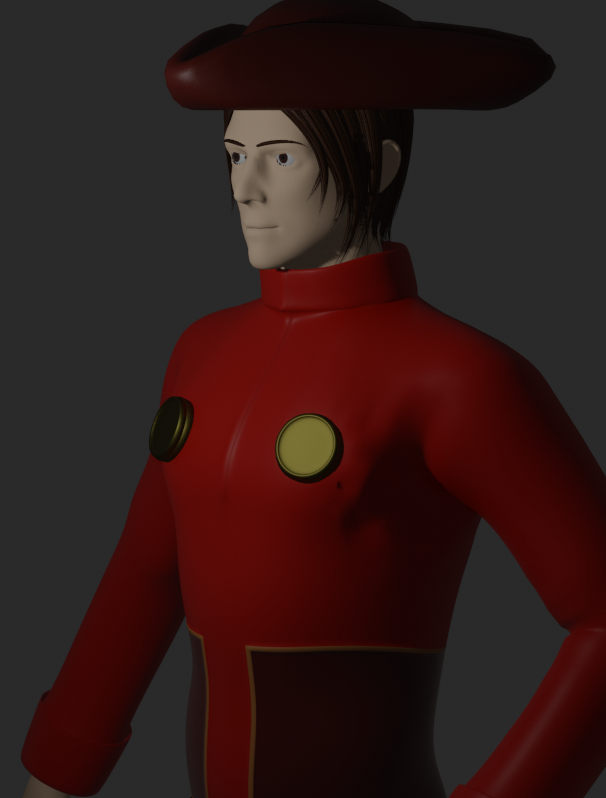
\includegraphics[width=\textwidth]{figures/Capitano.png}
%          \caption{Capitano}				% Questo ci ha permesso di concentrarci sulla fase di progettazione del corto, senza spendere tempo
%      \end{figure}									% nell'ideazione della storia.
%
%    \column{0.33\textwidth}
%      \begin{figure}
%          \centering
%          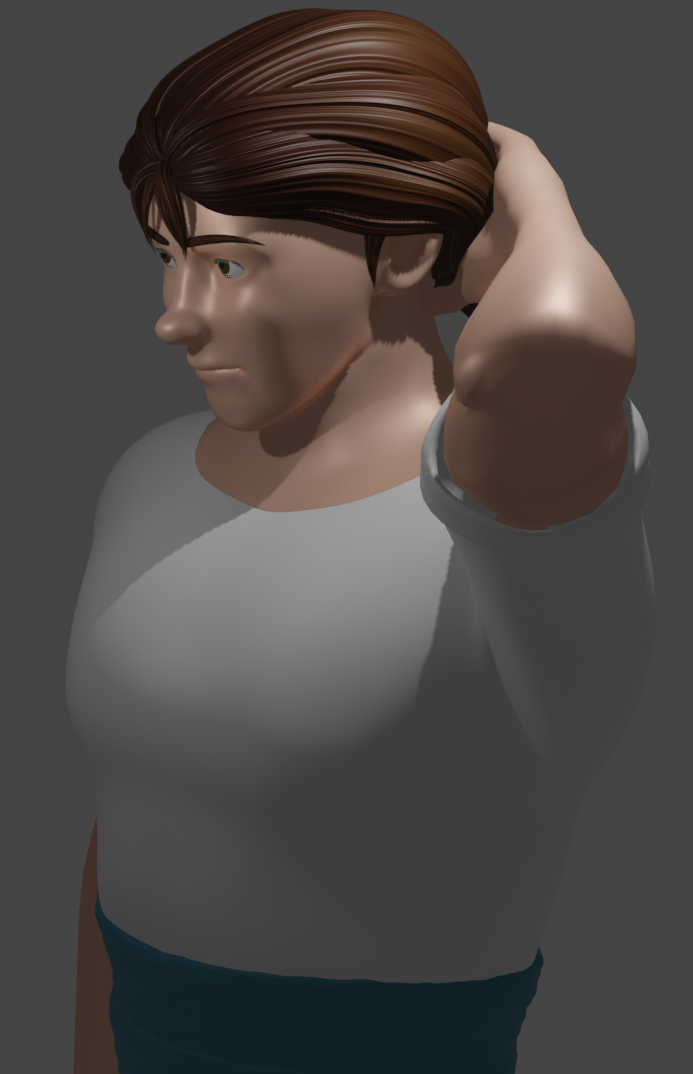
\includegraphics[width=\textwidth]{figures/ragazzo.png}
%          \caption{Ragazzo}
%      \end{figure}
%
%    \column{0.33\textwidth}
%      \begin{figure}
%          \centering
%          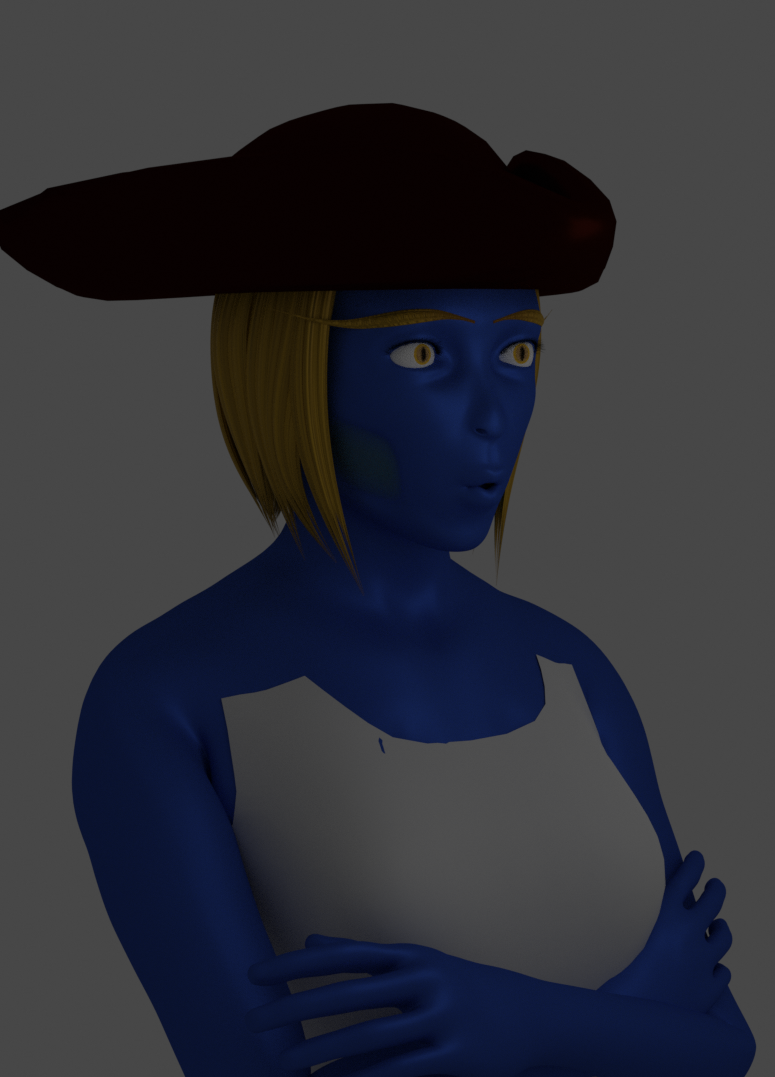
\includegraphics[width=\textwidth]{figures/Capitana.png}
%          \caption{Capitana}
%      \end{figure}
%  \end{columns}
%\end{frame}

\section{Concetti di animazione}										% Come ho già detto, sono state usate diverse tecniche di animazione,
                                             				% Ne vengono quindi spiegati alcuni concetti.
\begin{frame}{Rappresentazioni di rotazione}				% Le rotazioni coprono un ruolo fondamentale nelle animazioni, ne sono state usate principalmente 3:
  \begin{columns}[T,onlytextwidth]									% Angoli di Eulero, Quaternioni e Rappresentazione matriciale.
    \column{0.33\textwidth}
    \alert<1>{Angoli di Eulero}
      \begin{itemize}
							\item Concettualmente semplice							% La prima è quella concettualmente più semplice: utilizza 3 rotazioni una per ogni asse (X, Y e Z)
        \item Complessa e confusa in pratica							% L'implementazione però è complessa:
        \item L'ordine delle rotazioni è importante				% È importante stabilire l'ordine di queste tre rotazioni: cambiandolo cambia anche il risultato
        \item Gimbal lock e interpolazioni spezzate				% Inoltre, essendo gli assi dipendenti tra loro, questo modello presenta un problema, ovvero
      \end{itemize}										% che se due assi si allienano si perde un grado di libertà di rotazione. Questo problema è conosciuto come Gimbal Lock.

    \column{0.33\textwidth}
    \alert<2>{Quaternioni}
      \begin{itemize}
        \item No gimbal lock												% I quaternioni risolvono il problema presente nella rapresentazione euleriana.
				\item Concettualmente complessa							% Il costo è che questo modello risulta concettualmente più complesso, infatti una rotazione completa consiste in un angolo di 720°
        \item Semplifica i calcoli									% Ha però il vantagigo aggiuntivo di semplificare i calcoli
        \item Interpolazioni consistenti e dirette  % e il risultato sono interpolazioni dirette, non spezzate sui 3 assi.
      \end{itemize}
      
    \column{0.33\textwidth}
    \alert<3>{Matrici}																			% In fine la rappresentazione con l'uso di matrici
      \begin{itemize}						% permette di rappresentare qualsiasi tipo di trasformazione, non solo rotazioni.
				\item Qualsiasi tipo di trasformazione	% Sono concettualmente più complesse dei quaternioni, per questo motivo non vengono solitamente usate dall'utente finale (animatore)
				\item Parenting				% In blender ad esempio, esse sono utilizzate internamente, ogni rotazione viene convertita in matrice. Vengono anche usate per associazioni padre-figlio,
        \item Constraints			% vincoli
				\item Armature deform	% e deformazioni per l'uso di armature che permettono l'animazione di figure complesse come quella umana.
      \end{itemize}
  \end{columns}
\end{frame}

\begin{frame}{FK (Forward Kinematics)}					% Data la presenza di diversi personaggi, una delle tecniche maggiormente utilizzata è stata quella delle cinematiche,
  \begin{columns}[T,onlytextwidth]
    \column{0.5\textwidth}
		\begin{itemize}[<+- | alert@+>]							% che permettodo appunto di animare figure complesse, come quella umana.
      \item Figure complesse come quella umana  % ne esistono di due tipi. La cinematica diretta ha un approccio più naive ovvero, per posizionare un arto, viene applicata una rotazione
      \item Approccio naive											% ad ogni articolazione, partendo da quelle più vicine alla radice, che influenzano anche quelle più in basso nella gerarchia.
      \item Precisione del posizionamento				% Permette un posizionamento della figura molto preciso
      \item Difficile animare azioni comuni			% ma rende difficile animare azioni comuni siccome ruotare la spalla sposterebbe la posizione della mano.
    \end{itemize}
    \column{0.5\textwidth}
    \begin{figure}
      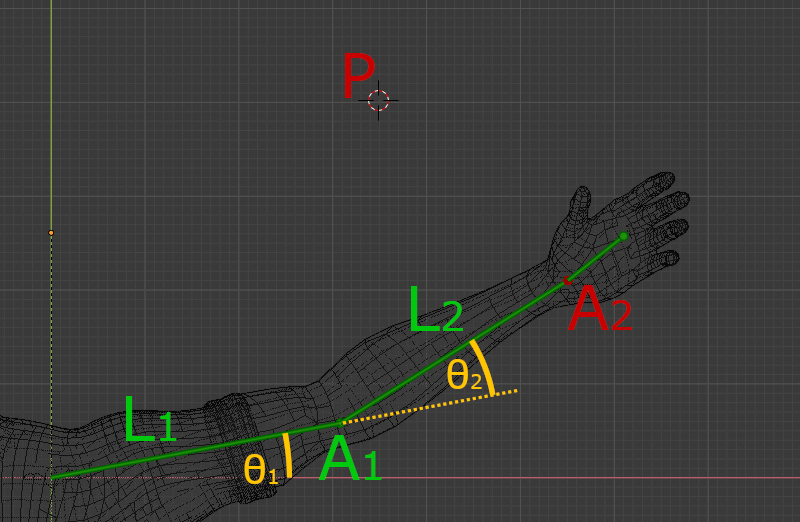
\includegraphics[width=.9\linewidth]{figures/17}
    \end{figure}
  \end{columns}
\end{frame}

\begin{frame}{IK (Inverse Kinematics)}					
  \begin{columns}[T,onlytextwidth]
    \column{0.5\textwidth}
		\begin{itemize}[<+- | alert@+>]							
    \item Approccio inverso											% La cinematica inversa ha un approccio opposto rispetto alla precedente.
    \item Figure complesse come quella umana		% Anch'essa, viene uilizzata per animare figure complesse ma,
		\item Semplifica le animazioni							% poiché viene posizionata diretamente l'ultima articolazione della gerarchia, e le altre vengono calcolte di conseguenza,
    \item Complessa da calcolare                % semplifica il lavoro dell'animatore, che non deve riposizionare la mano ogni volta che la spalla di un personaggio viene ruotata.
  \end{itemize}                                 % Ovviamente è più complessa da calcolare rispetto a quella diretta. Per farlo esistono diverse tecniche.
    \column{0.5\textwidth}
    \begin{figure}
      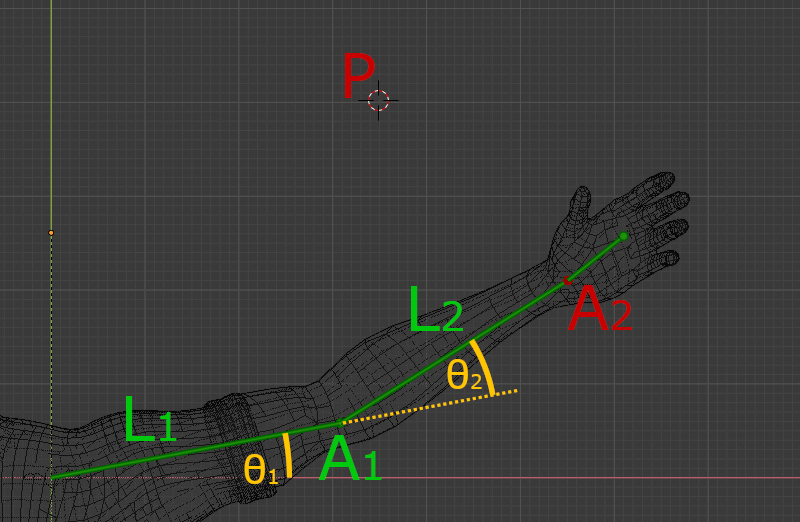
\includegraphics[width=.9\linewidth]{figures/17}
    \end{figure}
  \end{columns}
\end{frame}


\begin{frame}[fragile]{IK - Lo Jacobiano}				
  \alt<8>{
    \begin{align*}
        V &= J\dot{\theta}\\
        J^{-1}V &= \dot{\theta}
    \end{align*}
  }
  {
    \begin{columns}[onlytextwidth]
      \column{0.4\textwidth}
      \only<1-5>{
        $
        \begin{bmatrix}
            \dfrac{\partial p_x}{\partial \theta_1} & \dfrac{\partial p_x}{\partial \theta_2} & \dots & \dfrac{\partial p_x}{\partial \theta_n} \\[2ex]
            \dfrac{\partial p_y}{\partial \theta_1} & \dfrac{\partial p_y}{\partial \theta_2} & \dots & \dfrac{\partial p_y}{\partial \theta_n} \\[2ex]
            \vdots & \vdots & \ddots & \vdots \\[2ex]
            \dfrac{\partial \alpha_z}{\partial \theta_1} & \dfrac{\partial \alpha_z}{\partial \theta_2} & \dots & \dfrac{\partial \alpha_z}{\partial \theta_n} 
        \end{bmatrix}
        $
      }
      \only<6>{
        \begin{figure}
          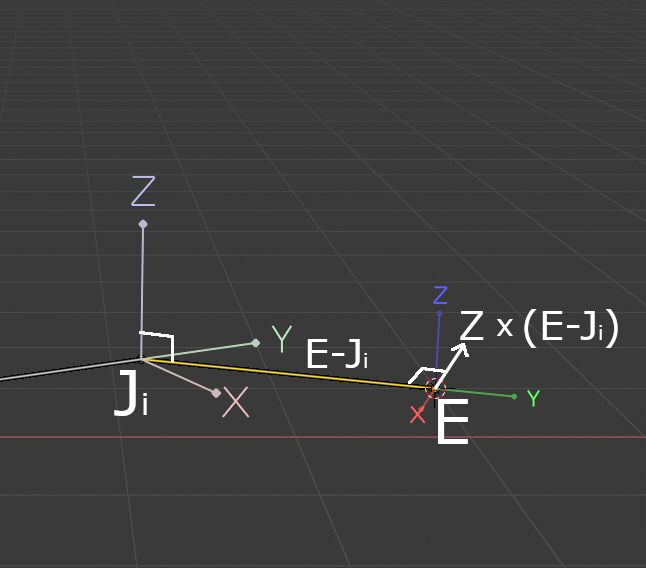
\includegraphics[width=.9\linewidth]{figures/16b}
          \caption{Velocità lineare, $v$}
        \end{figure}
      }
      \only<7>{
        \begin{figure}
          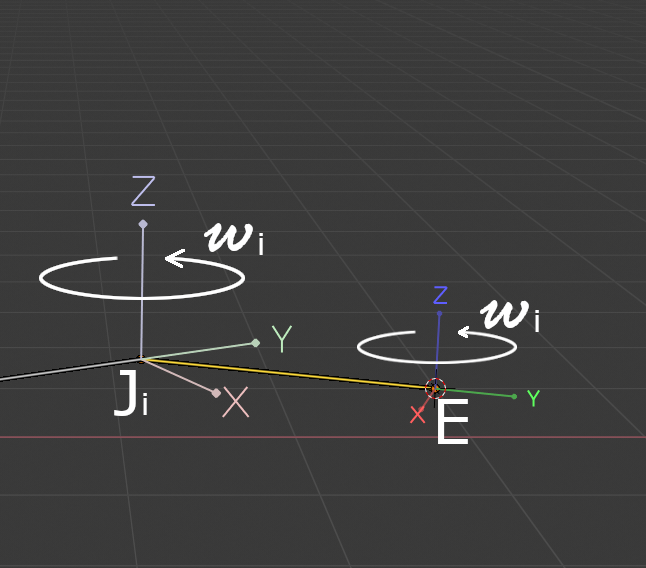
\includegraphics[width=.9\linewidth]{figures/16a}
          \caption{Velocità angolare, $\omega$}
        \end{figure}
      }
      \column{0.6\textwidth}											% La maggior parte di esse utilizza lo Jacobiano, ovvero una matrice...
      \only<1>{
        Matrice di derivate parziali corrispondenti alla differenza della posizione attuale dell'end-effector rispetto alla posizione obiettivo.
        \begin{alertblock}{Proprietà}	
            \begin{itemize}													% questo permette di calcolare iterativamente la posizione dell'end-effector (mano)
            \item Soluzione iterativa								% che si avvicina alla posizione obiettivo finché non la raggiunge, se esiste una soluzione
            \item Simile al simplesso		% Il metodo in cui la soluzione è calcolata è quindi simile a quello del simplesso.
          \end{itemize}
        \end{alertblock}
      }
      \only<2->{
        \begin{itemize}
          \item<2->
            \only<2-4>{$Y=
            \begin{bmatrix}
              p_x & p_y & p_z & \alpha_x & \alpha_y & \alpha_z
            \end{bmatrix}^T$}
            \only<5>{\alert{$
              V=
              \begin{bmatrix}
                  v_x & v_y & v_z & \omega_x & \omega_y & \omega_z
              \end{bmatrix}
              ^T
            $}}
            \only<6->{
              $v=Z\times(E-J_i)$ 
            }
            
          \item<3->
            \only<3-5>{$\dot{\theta}=
            \begin{bmatrix}
              \dot{\theta}_1 & \dot{\theta}_2 & \ldots & \dot{\theta}_n
            \end{bmatrix}^T$}
            \only<7>{
              $\omega=\omega_i$ 
            }
          \item<4-5>$V = \dot{Y} = J(\theta)\dot{\theta}$
        \end{itemize}
      }
    \end{columns}
  }
\end{frame}


\section{Progettazione}	% Affinché un modello 3D sia animabile, è necessario aggiungergli dei controlli per poterlo muovere.
\begin{frame}{Rigging}	% Questi sono comunemente chiamati rig, e devono essere progettati secondo le animazioni da realizzare.
  \begin{table}					% A tal proposito il rig è stato suddiviso in sotto-porzioni e, per ognuna sono state individuate le azioni 
					\caption{Diversi tipi di rig necessari un una figura umana in base ai compiti che deve eseguire}
		\begin{tabular}{lcr}% che essa dovrà eseguire. La soluzione di progettazione è stata scelta di conseguenza.
			\toprule
			Porzione del rig & Compito & Soluzione\\
			\midrule
			Braccia & raggiungere e gesticolare & IK e FK\\
			Mani & afferrare & FK\\
			Gambe & correre e camminare & IK\\
			\bottomrule
		\end{tabular}
	\end{table}	
  \begin{columns}[T,onlytextwidth]
    \column{0.33\textwidth}
    \begin{figure}
      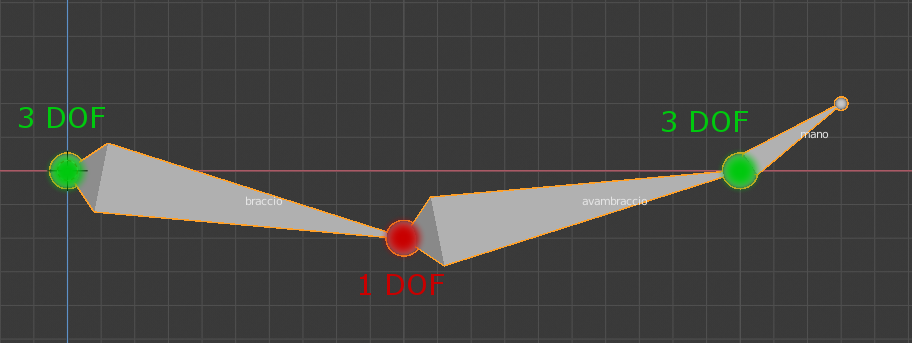
\includegraphics[width=.9\linewidth]{figures/arm}
    \end{figure}
    \column{0.33\textwidth}
    \begin{figure}
      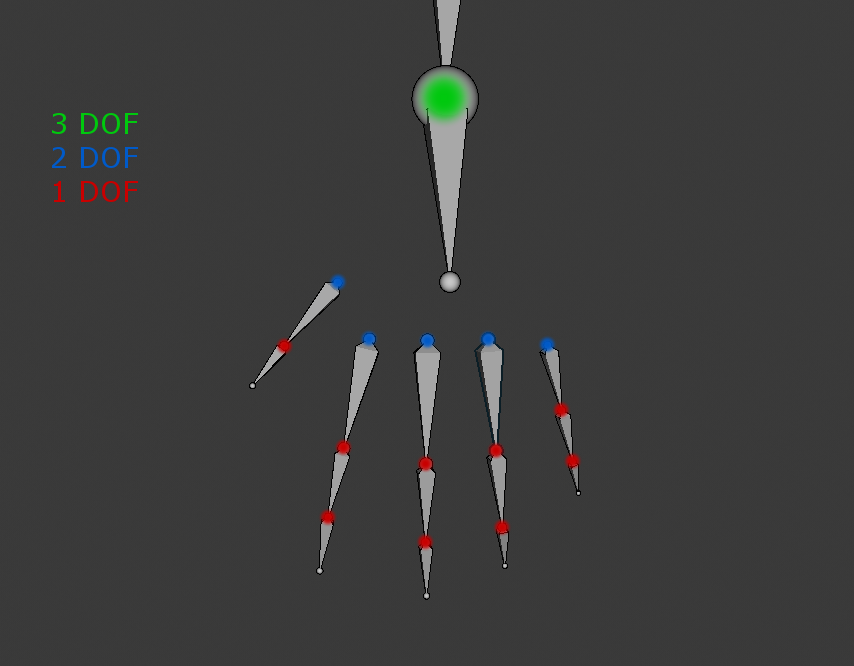
\includegraphics[width=.9\linewidth]{figures/hand}
    \end{figure}
    \column{0.33\textwidth}
    \begin{figure}
      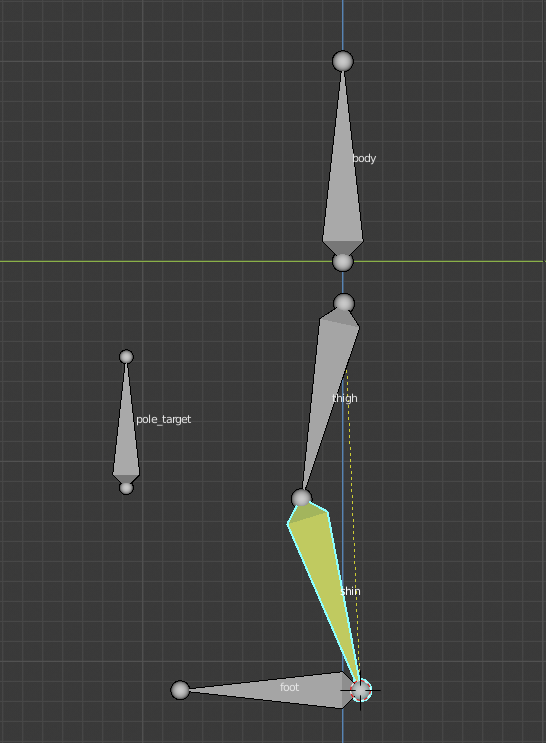
\includegraphics[width=.9\linewidth]{figures/leg}
    \end{figure}
  \end{columns}
\end{frame}

\section{Produzione}        % Nella produzione del cortometraggio è stato fatto uso di diverse animazioni già citate in precedenza.
\begin{frame}{Animazioni}   % Oltre alla cinematica diretta e inversa, alcune animazioni sono state rese cicliche.
	\metroset{block=fill}             % Ciò ha permesso di modularizzarle e riutilizzarle.
	\begin{columns}[T,onlytextwidth]  % Le curve sono state principalmente utilizzate come percorso di movimento.
                                    % In combinazione con animazioni cicliche, sul posto,
		\column{0.45\textwidth}         % esse hanno permesso di separare l'animazione dal movimento lungo la curva. 
    \begin{exampleblock}{IK}
		camminata\\
		corsa\\
		raggiungere
		\end{exampleblock}
		\begin{exampleblock}{FK}
		raggiungere\\
		afferrare
		\end{exampleblock}

		\column{0.45\textwidth}
		\begin{exampleblock}{Curve}
		camminata\\
		corsa\\
		inseguimento spaziale
		\end{exampleblock}
		\begin{exampleblock}{Cicli}
		camminata\\
		corsa\\
		sparatorie
		\end{exampleblock}
	\end{columns}
\end{frame}

{\setbeamercolor{palette primary}{fg=orange}
\begin{frame}[standout]

Risultato

\end{frame}
}

\end{document}
